\input{configTD.tex}

\usepackage{tikz, pgf}
\usetikzlibrary{arrows.meta, positioning, calc}
\newcommand{\R}{\mathbb{R}}
\newcommand{\N}{\mathbb{N}}

\title{Marches aléatoires sur un graphe et diagonalisation}
\author{}
\date{}

\begin{document}
\maketitle

\noindent\textbf{Objectif.}
Modéliser des situations concrètes par des marches aléatoires sur un graphe, écrire la matrice de transition associée, et utiliser la diagonalisation pour comprendre l'évolution du système et son état d'équilibre.

\medskip
 
% \noindent\textbf{Cadre général.}
% On considère un système qui peut se trouver dans un nombre fini d'\emph{états} (zones d'un bâtiment, niveaux d'un parking, etc.). À chaque pas de temps, le système passe d'un état à un autre selon des probabilités fixées. On note $P_{ij}$ la probabilité de passer de l'état $i$ à l'état $j$, et on rassemble ces nombres dans une matrice $P$ appelée \textbf{matrice de transition}. Si $\pi_n$ est le vecteur \emph{ligne} contenant la probabilité d'être dans chaque état à l'instant $n$, on a la relation fondamentale
% \[
%   \pi_{n+1} = \pi_n P, \qquad \text{donc} \qquad \pi_n = \pi_0 P^n.
% \]
% Calculer $P^n$ — et donc diagonaliser $P$ — permet de comprendre l'évolution du système au cours du temps et de trouver son état d'équilibre.

\vspace{1.5em}
\hrule
\vspace{1em}

%% ============================================================
%%  EXERCICE 1 — VISITEURS DANS UN MUSÉE (très guidé)
%% ============================================================
\section*{Exercice 1 : Répartition des visiteurs dans un musée}

\medskip

\begin{center}
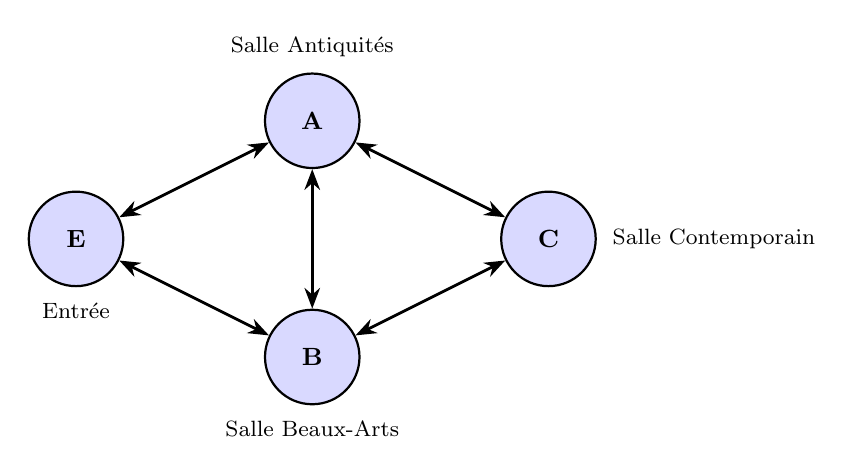
\begin{tikzpicture}[>=Stealth, thick, scale=1.0,
    salle/.style={circle, draw, fill=blue!15, minimum size=1.2cm, font=\small\bfseries}]
  \node[salle] (E) at (0,0) {E};
  \node[salle] (A) at (3,1.5) {A};
  \node[salle] (B) at (3,-1.5) {B};
  \node[salle] (C) at (6,0) {C};

  \draw[<->, line width=1pt] (E) -- (A);
  \draw[<->, line width=1pt] (E) -- (B);
  \draw[<->, line width=1pt] (A) -- (B);
  \draw[<->, line width=1pt] (A) -- (C);
  \draw[<->, line width=1pt] (B) -- (C);

  \node[below=2pt of E, font=\footnotesize] {Entrée};
  \node[above=2pt of A, font=\footnotesize] {Salle Antiquités};
  \node[below=2pt of B, font=\footnotesize] {Salle Beaux-Arts};
  \node[right=2pt of C, font=\footnotesize] {Salle Contemporain};
\end{tikzpicture}
\end{center}

\medskip

Un petit musée comporte quatre zones reliées par des passages comme indiqué sur le plan ci-dessus : l'\textbf{E}ntrée, la salle des \textbf{A}ntiquités, la salle des \textbf{B}eaux-Arts et la salle d'art \textbf{C}ontemporain. On observe les visiteurs toutes les 10 minutes et on note dans quelle zone ils se trouvent. À chaque pas de temps, un visiteur choisit \emph{au hasard et de manière équiprobable} l'un des passages partant de la zone où il se trouve, et l'emprunte.

\medskip

\begin{enumerate}[label=\alph*), itemsep=0.6em]
  \item Pour chaque zone, indiquer le nombre de zones voisines (c'est-à-dire le nombre de passages qui en partent).

\begin{solution}
$\mathrm{E}$ a 2 voisins (A et B). $\mathrm{A}$ a 3 voisins (E, B, C). $\mathrm{B}$ a 3 voisins (E, A, C). $\mathrm{C}$ a 2 voisins (A et B).
\end{solution}

  \item En déduire la \textbf{matrice de transition} $P$ du système, où $P_{ij}$ est la probabilité de passer de la zone $i$ à la zone $j$ en un pas de temps. On rangera les zones dans l'ordre $\mathrm{E}, \mathrm{A}, \mathrm{B}, \mathrm{C}$.

\begin{solution}
Depuis E, le visiteur va en A ou B avec probabilité $1/2$ chacun. Depuis A, il va en E, B ou C avec probabilité $1/3$ chacun. De même pour B. Depuis C, il va en A ou B avec probabilité $1/2$ chacun.
\[
  P = \begin{pmatrix}
    0 & 1/2 & 1/2 & 0 \\
    1/3 & 0 & 1/3 & 1/3 \\
    1/3 & 1/3 & 0 & 1/3 \\
    0 & 1/2 & 1/2 & 0
  \end{pmatrix}.
\]
\end{solution}

  \item Vérifier que la \textbf{somme de chaque ligne} de $P$ vaut 1. Pourquoi est-ce normal ?

\begin{solution}
Chaque ligne somme à 1 car, partant d'une zone donnée, le visiteur \emph{doit} aller quelque part : la somme des probabilités de toutes les destinations possibles vaut nécessairement 1. Une telle matrice est dite \textbf{stochastique}.
\end{solution}

  \item À l'instant $n = 0$, tous les visiteurs viennent d'entrer : $\pi_0 = (1, 0, 0, 0)$ (ligne). Calculer $\pi_1 = \pi_0 P$ et $\pi_2 = \pi_1 P$. Interpréter.

\begin{solution}
$\pi_1 = (0,\ 1/2,\ 1/2,\ 0)$ : après 10 minutes, la moitié des visiteurs est en A, l'autre moitié en B. C'est cohérent : depuis l'entrée, on n'a que ces deux choix.

$\pi_2 = \pi_1 P = (1/2 \cdot 1/3 + 1/2 \cdot 1/3,\ 1/2 \cdot 0 + 1/2 \cdot 1/3,\ 1/2 \cdot 1/3 + 1/2 \cdot 0,\ 1/2 \cdot 1/3 + 1/2 \cdot 1/3)$
$= (1/3,\ 1/6,\ 1/6,\ 1/3)$.

Après 20 minutes, un tiers des visiteurs est revenu à l'entrée, un tiers a atteint la salle d'art contemporain, et le reste se partage entre A et B.
\end{solution}

  \item On cherche maintenant la \textbf{distribution stationnaire} $\pi^\star$, c'est-à-dire un vecteur ligne de probabilités vérifiant $\pi^\star P = \pi^\star$ (la répartition n'évolue plus). Écrire le système linéaire correspondant et le résoudre, en n'oubliant pas la condition de normalisation $\pi_E^\star + \pi_A^\star + \pi_B^\star + \pi_C^\star = 1$.

\begin{solution}
Le système $\pi^\star P = \pi^\star$ s'écrit, en notant $\pi^\star = (e, a, b, c)$ :
\[
\begin{cases}
  e = a/3 + b/3, \\
  a = e/2 + b/3 + c/2, \\
  b = e/2 + a/3 + c/2, \\
  c = a/3 + b/3.
\end{cases}
\]
Par symétrie du problème entre A et B, on cherche une solution avec $a = b$. La première équation donne alors $e = 2a/3$, et la dernière $c = 2a/3$. La normalisation $e + 2a + c = 1$ donne $2a/3 + 2a + 2a/3 = 1$, soit $10a/3 = 1$, d'où $a = 3/10$.

Finalement :
\[
  \pi^\star = \left( \tfrac{2}{10},\ \tfrac{3}{10},\ \tfrac{3}{10},\ \tfrac{2}{10} \right) = (0{,}2\ ;\ 0{,}3\ ;\ 0{,}3\ ;\ 0{,}2).
\]
À long terme, 20\,\% des visiteurs sont en moyenne dans l'entrée, 20\,\% dans l'art contemporain, et 30\,\% dans chacune des deux salles intermédiaires.
\end{solution}

  \item Pouvait-on déduire les zones les plus fréquentées directement en observant le plan du musée ?

\begin{solution}

Oui, plus une zone a de salle voisine, plus elle est fréquentée. 

Détails mathématiques (pour les plus avancés) :

Notons $d_i$ le nombre de voisins du sommet $i$ et posons $\pi_i^\star = d_i / D$ avec $D = \sum_j d_j$. Vérifions que $\pi^\star P = \pi^\star$ : la composante en $j$ de $\pi^\star P$ vaut
\[
  \sum_i \pi_i^\star P_{ij} = \sum_{i \sim j} \frac{d_i}{D} \cdot \frac{1}{d_i} = \frac{1}{D} \sum_{i \sim j} 1 = \frac{d_j}{D} = \pi_j^\star.
\]
(La somme porte sur les voisins $i$ de $j$, qui sont au nombre de $d_j$.) C'est bien la distribution stationnaire. Ici $D = 2 + 3 + 3 + 2 = 10$, ce qui redonne $\pi^\star = (2/10, 3/10, 3/10, 2/10)$.

\end{solution}
  \item \textbf{Approche spectrale.} Diagonaliser $P$ : calculer ses valeurs propres, déterminer une base de vecteurs propres, puis écrire la décomposition $P = QDQ^{-1}$.

\begin{solution}
On trouve le polynôme caractéristique
\[
\chi_P(\lambda)=\lambda(\lambda-1)(3\lambda+1)(3\lambda-2),
\]
d'où les valeurs propres
\[
\lambda_1=1,\quad \lambda_2=-\frac23,\quad \lambda_3=-\frac13,\quad \lambda_4=0.
\]
Elles sont toutes distinctes, donc $P$ est diagonalisable.

Une base possible de vecteurs propres à droite est :
\[
v_1=\begin{pmatrix}1\\1\\1\\1\end{pmatrix} \ (\lambda=1),\quad
v_2=\begin{pmatrix}1\\-1\\-1\\1\end{pmatrix} \ (\lambda=-2/3),\quad
v_3=\begin{pmatrix}0\\1\\-1\\0\end{pmatrix} \ (\lambda=-1/3),\quad
v_4=\begin{pmatrix}1\\0\\0\\-1\end{pmatrix} \ (\lambda=0).
\]
En posant $Q=(v_1\ v_2\ v_3\ v_4)$ et
\[
D=\mathrm{diag}\!\left(1,-\frac23,-\frac13,0\right),
\]
on a bien $P=QDQ^{-1}$.
\end{solution}

  \item \textbf{Lien avec la distribution stationnaire et vitesse de convergence.}
  Expliquer pourquoi la distribution stationnaire est liée à la valeur propre $1$, puis interpréter la \emph{deuxième valeur propre en module} comme indicateur de la vitesse de convergence vers l'équilibre.

\begin{solution}
Pour une chaîne de Markov, la distribution stationnaire $\pi^\star$ vérifie
\[
\pi^\star P=\pi^\star,
\]
donc $\pi^\star$ est un vecteur propre \emph{à gauche} associé à la valeur propre $1$.
Ici on retrouve bien $\pi^\star=(0{,}2,\,0{,}3,\,0{,}3,\,0{,}2)$.

Dans la décomposition spectrale de $P^n$, le mode associé à $\lambda=1$ est le mode permanent (la limite), tandis que les autres modes sont transitoires et sont multipliés par $\lambda^n$.

La plus grande valeur propre en module après $1$ vaut ici
\[
|\lambda_2|=\frac23.
\]
L'écart à l'équilibre décroît donc globalement comme $\left(\frac23\right)^n$ (avec alternance possible de signe car $\lambda_2<0$). Plus $|\lambda_2|$ est proche de 1, plus la convergence est lente.
\end{solution}
\end{enumerate}

\medskip
\noindent\textbf{Question d'ouverture.} Si l'on voulait \emph{augmenter} la fréquentation de la salle d'art contemporain (la moins visitée avec l'entrée), que pourrait-on modifier dans le plan du musée ? Comment cela se traduirait-il sur la matrice $P$ et sur $\pi^\star$ ?

\vspace{1em}

\medskip
\noindent\fbox{%
\parbox{0.97\linewidth}{%
\textbf{Encadré théorique (théorème de Perron-Frobenius).)}
Si $P$ est une matrice stochastique (sommes des lignes égales à 1), alors $1$ est toujours une valeur propre simple de $P$.
Il existe un vecteur propre associé à cette valeur propre avec tous les coefficients positifs et dont la somme vaut 1.

Les autres valeurs propres ont un module strictement inférieur à 1.
}%
}

\vspace{1.5em}
\hrule
\vspace{2em}


%% ============================================================
%%  EXERCICE 2 — ENGINS DE CHANTIER (avec diagonalisation)
%% ============================================================
\section*{Exercice 2 : Rotation des engins sur un chantier}

\medskip

\begin{center}
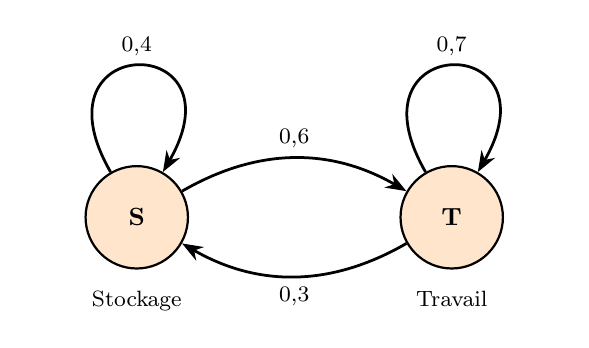
\begin{tikzpicture}[>=Stealth, thick, scale=1.0,
    zone/.style={circle, draw, fill=orange!20, minimum size=1.3cm, font=\small\bfseries}]
  \node[zone] (S) at (0,0) {S};
  \node[zone] (T) at (4,0) {T};

  \draw[->, line width=1pt] (S) to[out=30, in=150] node[above, font=\footnotesize] {$0{,}6$} (T);
  \draw[->, line width=1pt] (T) to[out=210, in=-30] node[below, font=\footnotesize] {$0{,}3$} (S);
  \draw[->, line width=1pt] (S) to[out=120, in=60, looseness=8] node[above, font=\footnotesize] {$0{,}4$} (S);
  \draw[->, line width=1pt] (T) to[out=120, in=60, looseness=8] node[above, font=\footnotesize] {$0{,}7$} (T);

  \node[below=4pt of S, font=\footnotesize] {Stockage};
  \node[below=4pt of T, font=\footnotesize] {Travail};
\end{tikzpicture}
\end{center}

\medskip

Sur un chantier, une flotte de camions-bennes effectue des rotations entre deux zones : la zone de \textbf{S}tockage des matériaux et la zone de \textbf{T}ravail (où l'on coule le béton). On observe la position des camions toutes les 30 minutes. Une étude statistique du chantier a permis d'estimer les probabilités de transition suivantes : un camion en zone S y reste avec probabilité $0{,}4$ et part en zone T avec probabilité $0{,}6$ ; un camion en zone T y reste avec probabilité $0{,}7$ et retourne en zone S avec probabilité $0{,}3$.

\medskip
\begin{enumerate}[label=\alph*), itemsep=0.6em]
  \item Écrire la matrice de transition $P$ du système (lignes : S puis T).

\begin{solution}
\[
  P = \begin{pmatrix} 0{,}4 & 0{,}6 \\ 0{,}3 & 0{,}7 \end{pmatrix}.
\]
On vérifie que chaque ligne somme à 1.
\end{solution}

  \item Diagonaliser $P$ : calculer son polynôme caractéristique, ses valeurs propres et des vecteurs propres associés. On notera $Q$ la matrice de passage et $D$ la matrice diagonale.

\begin{solution}
$\chi_P(\lambda) = (0{,}4 - \lambda)(0{,}7 - \lambda) - 0{,}18 = \lambda^2 - 1{,}1\lambda + 0{,}28 - 0{,}18 = \lambda^2 - 1{,}1\lambda + 0{,}1 = (\lambda - 1)(\lambda - 0{,}1)$.

Valeurs propres : $\lambda_1 = 1$ et $\lambda_2 = 0{,}1$.

\textbf{Remarque importante.} La valeur propre $\lambda_1 = 1$ apparaît : c'est une propriété générale de toutes les matrices stochastiques (la somme des lignes vaut 1, donc le vecteur colonne $(1, 1)^\top$ est vecteur propre à droite associé à $1$).

Vecteur propre (à droite) pour $\lambda_1 = 1$ : $(P - I)V = 0$ donne $-0{,}6 v_1 + 0{,}6 v_2 = 0$, soit $V_1 = \begin{pmatrix} 1 \\ 1 \end{pmatrix}$.

Vecteur propre pour $\lambda_2 = 0{,}1$ : $(P - 0{,}1\, I)V = 0$ donne $0{,}3 v_1 + 0{,}6 v_2 = 0$, soit $V_2 = \begin{pmatrix} 2 \\ -1 \end{pmatrix}$.

D'où $Q = \begin{pmatrix} 1 & 2 \\ 1 & -1 \end{pmatrix}$ et $D = \begin{pmatrix} 1 & 0 \\ 0 & 0{,}1 \end{pmatrix}$.
\end{solution}

  \item En déduire l'expression de $P^n$ pour tout $n \in \N$.

\begin{solution}
On a $P = QDQ^{-1}$ donc $P^n = Q D^n Q^{-1}$. On calcule $Q^{-1} = \dfrac{1}{-3}\begin{pmatrix} -1 & -2 \\ -1 & 1 \end{pmatrix} = \dfrac{1}{3}\begin{pmatrix} 1 & 2 \\ 1 & -1 \end{pmatrix}$.
\[
P^n = \begin{pmatrix} 1 & 2 \\ 1 & -1 \end{pmatrix}
      \begin{pmatrix} 1 & 0 \\ 0 & (0{,}1)^n \end{pmatrix}
      \frac{1}{3}\begin{pmatrix} 1 & 2 \\ 1 & -1 \end{pmatrix}
= \frac{1}{3}\begin{pmatrix} 1 + 2(0{,}1)^n & 2 - 2(0{,}1)^n \\ 1 - (0{,}1)^n & 2 + (0{,}1)^n \end{pmatrix}.
\]
\end{solution}

  \item À l'instant $n = 0$, tous les camions sont au stockage : $\pi_0 = (1, 0)$. En déduire $\pi_n$ pour tout $n$, puis donner la limite quand $n \to +\infty$.

\begin{solution}
$\pi_n = \pi_0 P^n = $ première ligne de $P^n$, soit
\[
  \pi_n = \left( \tfrac{1 + 2(0{,}1)^n}{3},\ \tfrac{2 - 2(0{,}1)^n}{3} \right).
\]
Quand $n \to +\infty$, $(0{,}1)^n \to 0$, donc
\[
  \pi_n \longrightarrow \pi^\star = \left( \tfrac{1}{3},\ \tfrac{2}{3} \right) \approx (0{,}33\ ;\ 0{,}67).
\]
À long terme, en moyenne un tiers des camions est au stockage et deux tiers sont en zone de travail.
\end{solution}

  \item Vérifier que cette limite $\pi^\star$ satisfait bien $\pi^\star P = \pi^\star$.

\begin{solution}
$\pi^\star P = (1/3 \cdot 0{,}4 + 2/3 \cdot 0{,}3,\ 1/3 \cdot 0{,}6 + 2/3 \cdot 0{,}7) = (2/15 + 2/10,\ 2/10 + 14/30)$.

Premier terme : $2/15 + 3/15 = 5/15 = 1/3$. Second terme : $6/30 + 14/30 = 20/30 = 2/3$. \checkmark
\end{solution}

  \item \textbf{Vitesse de convergence.} À partir de quel instant $n$ la répartition est-elle à moins de $1\,\%$ de la répartition stationnaire ? Quel rôle joue la deuxième valeur propre $\lambda_2 = 0{,}1$ dans cette vitesse de convergence ?

\begin{solution}
L'écart à l'équilibre vaut, en valeur absolue sur la première composante, $\dfrac{2(0{,}1)^n}{3}$. On veut $\dfrac{2(0{,}1)^n}{3} \leq 0{,}01$, soit $(0{,}1)^n \leq 0{,}015$, donc $n \geq \log(0{,}015)/\log(0{,}1) \approx 1{,}8$.

Dès $n = 2$ (soit après 1 heure), la répartition est à moins de 1\,\% de l'équilibre. La convergence est très rapide car la deuxième valeur propre $\lambda_2 = 0{,}1$ est très petite devant 1 : le terme transitoire $(0{,}1)^n$ s'éteint en quelques pas.

\textbf{Règle générale :} la vitesse de convergence vers l'équilibre est gouvernée par $|\lambda_2|^n$, où $\lambda_2$ est la deuxième plus grande valeur propre en module. Plus $|\lambda_2|$ est proche de 1, plus la convergence est lente (le système ``met du temps à oublier'' son état initial).
\end{solution}
\end{enumerate}

\vspace{1.5em}
\hrule
\vspace{2em}

%% ============================================================
%%  EXERCICE 3 — PARKING (autonome, plus ouvert)
%% ============================================================

\section*{Exercice 3 : Occupation d'un parking à étages}

\medskip

Un parking de centre commercial comporte trois niveaux : le niveau \textbf{0} (rez-de-chaussée, accessible directement depuis la rue), le niveau \textbf{1} et le niveau \textbf{2}. Toutes les 5 minutes, on observe que les véhicules en mouvement se déplacent selon les probabilités suivantes :

\medskip

\begin{itemize}[nosep]
  \item Depuis le niveau 0 : $0{,}2$ y reste, $0{,}8$ monte au niveau 1.
  \item Depuis le niveau 1 : $0{,}3$ redescend au niveau 0, $0{,}3$ y reste, $0{,}4$ monte au niveau 2.
  \item Depuis le niveau 2 : $0{,}5$ redescend au niveau 1, $0{,}5$ y reste.
\end{itemize}

\medskip
\begin{enumerate}[label=\alph*), itemsep=0.6em]
  \item Représenter le graphe de transition du système (sommets = niveaux, arêtes orientées = transitions) et écrire la matrice de transition $P$ (lignes : niveau 0, 1, 2).

\begin{solution}
\[
  P = \begin{pmatrix}
    0{,}2 & 0{,}8 & 0 \\
    0{,}3 & 0{,}3 & 0{,}4 \\
    0 & 0{,}5 & 0{,}5
  \end{pmatrix}.
\]
\end{solution}

  \item Déterminer la distribution stationnaire $\pi^\star$ en résolvant directement $\pi^\star P = \pi^\star$ (avec normalisation).

\begin{solution}
Notons $\pi^\star = (p_0, p_1, p_2)$. Le système $\pi^\star P = \pi^\star$ donne :
\[
\begin{cases}
  p_0 = 0{,}2\, p_0 + 0{,}3\, p_1, \\
  p_1 = 0{,}8\, p_0 + 0{,}3\, p_1 + 0{,}5\, p_2, \\
  p_2 = 0{,}4\, p_1 + 0{,}5\, p_2.
\end{cases}
\]
La première équation donne $0{,}8\, p_0 = 0{,}3\, p_1$, soit $p_1 = \dfrac{8}{3}\, p_0$.

La troisième donne $0{,}5\, p_2 = 0{,}4\, p_1$, soit $p_2 = \dfrac{4}{5}\, p_1 = \dfrac{32}{15}\, p_0$.

Normalisation : $p_0 + p_1 + p_2 = 1$, soit $p_0\left(1 + \dfrac{8}{3} + \dfrac{32}{15}\right) = 1$.

Mise au même dénominateur : $p_0 \cdot \dfrac{15 + 40 + 32}{15} = 1$, donc $p_0 = \dfrac{15}{87} = \dfrac{5}{29}$.

D'où :
\[
  \pi^\star = \left( \tfrac{15}{87},\ \tfrac{40}{87},\ \tfrac{32}{87} \right) \approx (0{,}172\ ;\ 0{,}460\ ;\ 0{,}368).
\]
À long terme, environ 17\,\% des véhicules sont au niveau 0, 46\,\% au niveau 1 et 37\,\% au niveau 2.
\end{solution}

  \item Vérifier que $\lambda = 1$ est valeur propre de $P$ et donner un vecteur propre à droite associé. (\emph{Indication :} pensez aux sommes des lignes.)

\begin{solution}
Comme $P$ est stochastique, chaque ligne somme à 1, donc $P\begin{pmatrix} 1 \\ 1 \\ 1 \end{pmatrix} = \begin{pmatrix} 1 \\ 1 \\ 1 \end{pmatrix}$. Le vecteur $(1, 1, 1)^\top$ est vecteur propre à droite associé à la valeur propre $\lambda = 1$.
\end{solution}

  \item \textbf{Question ouverte.} Le directeur du parking constate que le niveau 0 est sous-utilisé. Il envisage de modifier la signalétique pour pousser plus de visiteurs à y rester (par exemple en augmentant la probabilité $0{,}2 \to 0{,}5$ de rester au niveau 0, et en réduisant $0{,}8 \to 0{,}5$ celle de monter au niveau 1). Recalculer la nouvelle distribution stationnaire et commenter.

\begin{solution}
Nouvelle matrice :
\[
  P' = \begin{pmatrix}
    0{,}5 & 0{,}5 & 0 \\
    0{,}3 & 0{,}3 & 0{,}4 \\
    0 & 0{,}5 & 0{,}5
  \end{pmatrix}.
\]
On résout $\pi^\star P' = \pi^\star$. La première équation devient $0{,}5\, p_0 = 0{,}3\, p_1$, soit $p_1 = \dfrac{5}{3}\, p_0$. La troisième est inchangée, $p_2 = \dfrac{4}{5}\, p_1 = \dfrac{4}{3}\, p_0$.

Normalisation : $p_0 \left(1 + \dfrac{5}{3} + \dfrac{4}{3}\right) = p_0 \cdot 4 = 1$, soit $p_0 = 1/4$.

\[
  \pi^\star = \left( \tfrac{1}{4},\ \tfrac{5}{12},\ \tfrac{4}{12} \right) \approx (0{,}25\ ;\ 0{,}417\ ;\ 0{,}333).
\]
Le taux d'occupation du niveau 0 passe d'environ 17\,\% à 25\,\%, ce qui est l'effet recherché. En contrepartie, les niveaux 1 et 2 sont un peu moins fréquentés. La modification a bien l'effet souhaité, mais pas de manière spectaculaire : la majorité des véhicules continue à monter, car la dynamique en chaîne (0 $\to$ 1 $\to$ 2) reste favorable aux étages supérieurs.
\end{solution}
\end{enumerate}


\vspace{1.5em}
\hrule
\vspace{2em}
\newpage

%% ============================================================
%%  EXERCICE 4 — LOGISTIQUE BTP (graphe plus complexe)
%% ============================================================

\section*{Exercice 4 : Flux logistique sur un grand chantier BTP}

\medskip

Sur un grand chantier de construction, on suit la position d'un camion-toupie toutes les 15 minutes. On distingue 6 zones :
\[
\mathrm{C}=\text{Centrale b\'eton},\quad
\mathrm{A}=\text{Acc\`es principal},\quad
\mathrm{G}=\text{Grue / zone de levage},
\]
\[
\mathrm{M}=\text{Zone ma\c connerie},\quad
\mathrm{F}=\text{Zone fondations},\quad
\mathrm{S}=\text{Zone stockage}.
\]

Le schéma de circulation est modélisé par le graphe orienté probabiliste ci-dessous.

\begin{center}
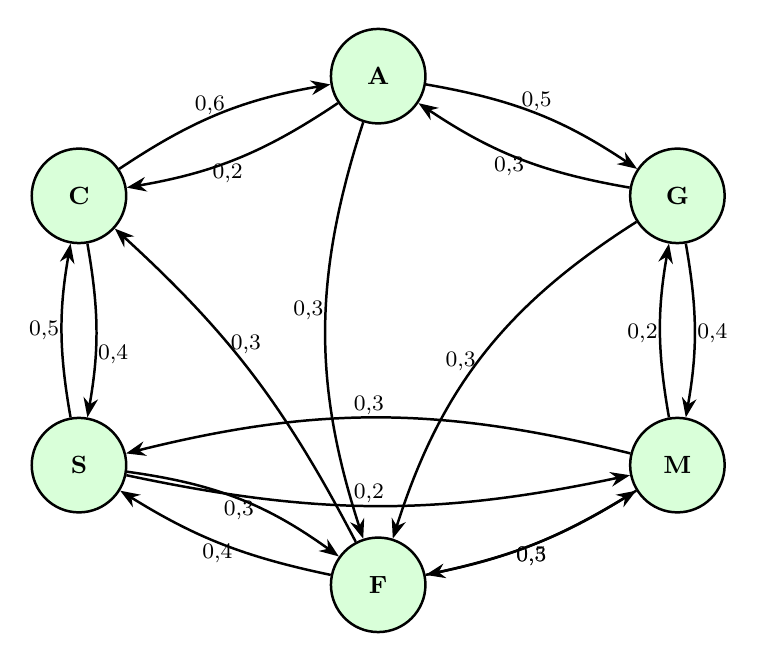
\begin{tikzpicture}[
  >=Stealth, line width=0.9pt, scale=0.95,
  zone/.style={circle, draw, fill=green!15, minimum size=1.2cm, font=\small\bfseries},
  prob/.style={font=\footnotesize,  inner sep=0.5pt}
]
  % Disposition en hexagone pour limiter les croisements visuels.
  \node[zone] (C) at (-4,1.8) {C};
  \node[zone] (A) at (0,3.4) {A};
  \node[zone] (G) at (4,1.8) {G};
  \node[zone] (M) at (4,-1.8) {M};
  \node[zone] (F) at (0,-3.4) {F};
  \node[zone] (S) at (-4,-1.8) {S};

  \draw[->] (C) to[bend left=12] node[prob, pos=0.45, above] {$0{,}6$} (A);
  \draw[->] (C) to[bend left=10] node[prob, pos=0.65, right] {$0{,}4$} (S);

  \draw[->] (A) to[bend left=12] node[prob, pos=0.50, above] {$0{,}5$} (G);
  \draw[->] (A) to[bend left=12] node[prob, pos=0.55, below] {$0{,}2$} (C);
  \draw[->] (A) to[bend right=18] node[prob, pos=0.45, left] {$0{,}3$} (F);

  \draw[->] (G) to[bend left=10] node[prob, pos=0.52, right] {$0{,}4$} (M);
  \draw[->] (G) to[bend left=12] node[prob, pos=0.55, below] {$0{,}3$} (A);
  \draw[->] (G) to[bend right=20] node[prob, pos=0.52, left] {$0{,}3$} (F);

  \draw[->] (M) to[bend left=10] node[prob, pos=0.52, below] {$0{,}5$} (F);
  \draw[->] (M) to[bend left=10] node[prob, pos=0.48, left] {$0{,}2$} (G);
  \draw[->] (M) to[bend right=14] node[prob, pos=0.52, above] {$0{,}3$} (S);

  \draw[->] (F) to[bend left=10] node[prob, pos=0.52, below] {$0{,}4$} (S);
  \draw[->] (F) to[bend right=10] node[prob, pos=0.6, right] {$0{,}3$} (C);
  \draw[->] (F) to[bend right=10] node[prob, pos=0.48, below] {$0{,}3$} (M);

  \draw[->] (S) to[bend left=10] node[prob, pos=0.50, left] {$0{,}5$} (C);
  \draw[->] (S) to[bend left=14] node[prob, pos=0.50, below] {$0{,}3$} (F);
  \draw[->] (S) to[bend right=12] node[prob, pos=0.48, above] {$0{,}2$} (M);
\end{tikzpicture}
\end{center}

\medskip
\begin{enumerate}[label=\alph*), itemsep=0.6em]
  \item Écrire la matrice de transition $P$ associée à cette évolution en prenant l'ordre des états
  \[
  (\mathrm{C},\mathrm{A},\mathrm{G},\mathrm{M},\mathrm{F},\mathrm{S}).
  \]

\begin{solution}
En lisant les probabilités sortantes de chaque sommet dans l'ordre demandé :
\[
P=
\begin{pmatrix}
0   & 0{,}6 & 0   & 0   & 0   & 0{,}4 \\
0{,}2 & 0   & 0{,}5 & 0   & 0{,}3 & 0   \\
0   & 0{,}3 & 0   & 0{,}4 & 0{,}3 & 0   \\
0   & 0   & 0{,}2 & 0   & 0{,}5 & 0{,}3 \\
0{,}3 & 0   & 0   & 0{,}3 & 0   & 0{,}4 \\
0{,}5 & 0   & 0   & 0{,}2 & 0{,}3 & 0
\end{pmatrix}.
\]
\end{solution}

  \item Vérifier que $P$ est bien stochastique, puis expliquer brièvement ce que représente l'entrée $P_{4,5}$ dans ce contexte.

\begin{solution}
Chaque ligne somme à 1, donc $P$ est une matrice stochastique.

L'entrée $P_{4,5}$ (ligne 4, colonne 5 dans l'ordre choisi) vaut $0{,}5$ : cela signifie qu'un camion situé en zone $\mathrm{M}$ (maçonnerie) a une probabilité de $50\,\%$ d'être en zone $\mathrm{F}$ (fondations) au pas de temps suivant.
\end{solution}

\item Quelles sont les étapes à suivre pour déterminer les endroits où le camion-toupie passera le plus de temps ?

\begin{solution}
On peut diagonaliser la matrice $P$ pour obtenir les valeurs propres et les vecteurs propres. Les endroits où le camion-toupie passera le plus de temps sont les endroits où la valeur propre est la plus grande.

On peut aussi utiliser la distribution stationnaire $\pi^\star$ pour obtenir les endroits où le camion-toupie passera le plus de temps. Les endroits où le camion-toupie passera le plus de temps sont les endroits où la probabilité est la plus grande.
\end{solution}

\end{enumerate}

\end{document}
